% This file contains all homework from week 38
% use \section{<name>}  to create a section per homework assignment

\section[Homework 4]{Homework 4: XUTools}

XUTools manipulate files in terms of language-specific constucts, like C functions, IOS interface blocks and XML elements.

XUTools presents eXtended Unix text-processing tool (XUTools) that enable extracting, counting and comparing in terms of language-specific constructs. The XUTools use a library of language grammars and xupath which is an xpath-like querying language to perform its operations. The following tools are considered the XUTools:

\begin{itemize}
	\item xugrep
	\item xuwc
	\item xudiff
\end{itemize}

\subsection{xugrep}

	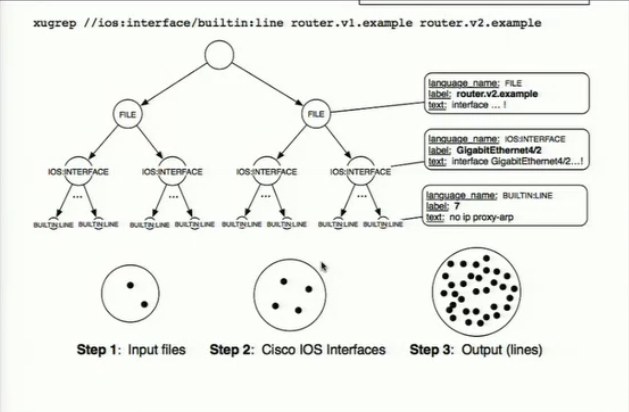
\includegraphics[scale=0.5]{xugrep}

\subsection{xuwc}

Xuwc makes it possible to count text by understanding the structure for a specific language. So xuwc basically understands to language hierarchy in order to perform its job, which is counting. 

       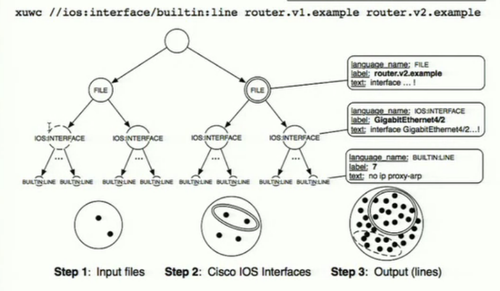
\includegraphics[scale=0.5]{xuwc}

\subsection{xudiff}

Xudiff compares two files in terms of higher-level-language constructs.

	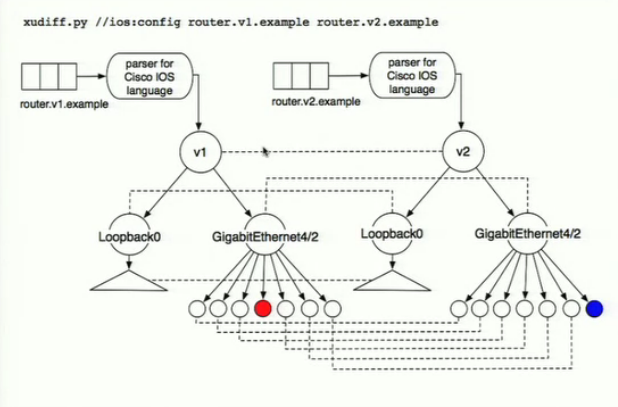
\includegraphics[scale=0.5]{xudiff}
